\documentclass{res/theme}
\usepackage{wallpaper}
\usepackage[dutch]{babel}
\usepackage{tabu,longtable,booktabs,array}
\def\changemargin#1#2{\list{}{\rightmargin#2\leftmargin#1}\item[]}
\let\endchangemargin=\endlist 
\newcommand{\block}[1]{\vspace{1.4cm}\begin{changemargin}{2.5cm}{2.5cm}\large\textit{#1}\end{changemargin}\vspace{0.6cm}}
\ThisCenterWallPaper{0.7}{res/cover.png}
\usepackage{microtype} % Better word wrapping
  \usepackage{color}
\usepackage{xcolor}
\usepackage{titlesec}
\usepackage{wrapfig}
\titleformat{\section}
  {\normalfont\Large}
  {\thesection}{1em}{}
\titleformat{\subsection}
  {\normalfont\large}
  {\thesection}{1em}{}
\usepackage{hyperref}
\definecolor{blue}{rgb}{0.01, 0.28, 1.0}
\definecolor{lightgray}{rgb}{0.95, 0.95, 0.95}
\hypersetup{colorlinks=true, urlcolor=blue, citecolor=blue, filecolor=blue, linkcolor=blue}
\usepackage{afterpage}
\pagecolor{lightgray}\afterpage{\nopagecolor}
\usepackage[firstpage=true]{background}
\usepackage{amsmath}
\newcommand{\stackeq}[1]{\overset{\text{\tiny #1}}{=}}
\def\Step{0.1cm}
\tikzset{dotted lines/.style={black, loosely dotted,  thick}}
\backgroundsetup{
scale=1,
angle=0,
position={0,0},
contents={
\begin{tikzpicture}[remember picture,overlay]
\draw[dotted lines,step=\Step,help lines]
  (-10,-30) grid  (20,10);
  \end{tikzpicture}
  }
}
\usepackage[font={footnotesize}]{caption}
\usepackage[ruled,vlined]{algorithm2e}
\newenvironment{snippet}[1][htb]
  {\renewcommand{\algorithmcfname}{Code Snippet}% Update algorithm name
   \vspace{0.3cm}\begin{algorithm}[#1]%
  }{\end{algorithm}\vspace{0.3cm}}
\usepackage{array}
\usepackage{tabu}
\usepackage{float}
\usepackage[all]{hypcap}
\usepackage{etoolbox}
\usepackage{xfrac}
\usepackage{fancyvrb}
\usepackage{listings}
\makeatletter
\patchcmd{\@BVerbatim}
  {\BVerbatim@font}
  {\BVerbatim@font\footnotesize}
  {}{}
\makeatother

%%%%%%%%%%%%%%%%%%%%%%%%%%%%%%%%%%%
%%%%%%%%%%%%%%%%%%%%%%%%%%%%%%%%%%%
%%%%%%%%%%%%%%%%%%%%%%%%%%%%%%%%%%%

%%% Authors
\addAuthor{Bruno}{Vandekerkhove}{}

%%% Title page
\casename{Practicum 1 - Lagerangbenaderingen}
\subtitle{Bruno Vandekerkhove}
\course{{G0Q57A: Modellering \& Simulatie}}
\academicyear{2019}
\newcommand{\tbd}{\textbf{To be discussed}}

%%%
%%% Start Document
%%%
\begin{document}
\maketitle
\tableofcontents

%
% Aanbevelingssysteem
% 

\fakesection{Een Aanbevelingssysteem voor Films}

\begin{center}
\textit{De broncode bevindt zich in de \texttt{src} folder. Het algemene script (\texttt{src/s0216676\_script}) is opgedeeld in secties, \'e\'en per opgave. Elke opgave wordt hieronder afzonderlijk beantwoord. Aan het einde van elk antwoord wordt (indien nodig) de broncode weergegeven.}
\end{center}

%%%
%%%
%%%

\fakesubsection{Opdracht 1}

We laden de dataset in met de \texttt{load} functie. De uitvoer staat weergegeven in figuur \ref{fig:op1}.

\vspace{0.3cm}
\begin{figure}[h]
\centering
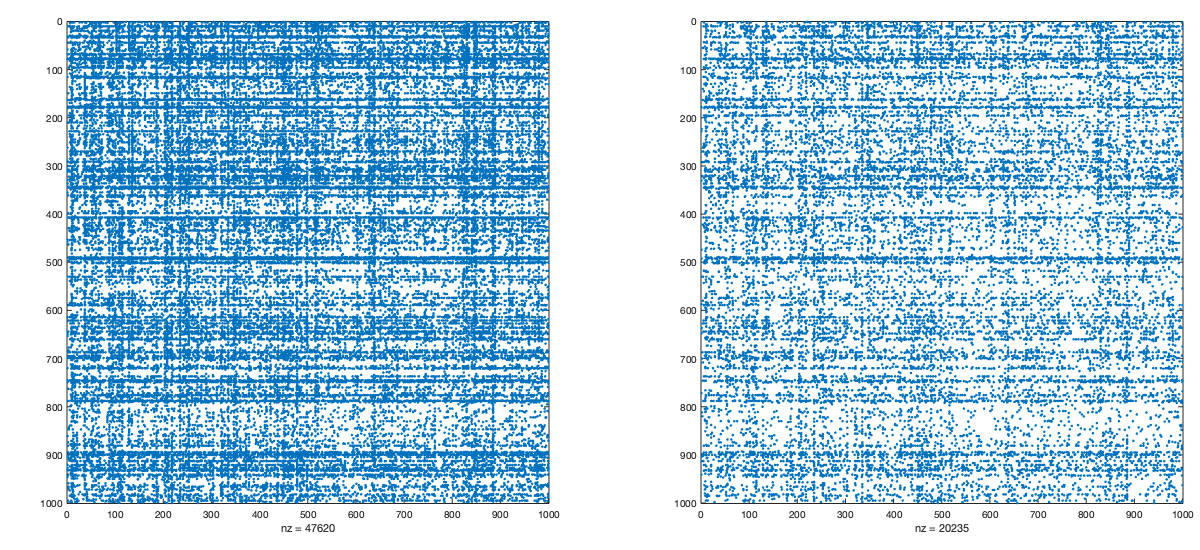
\includegraphics[width=0.5\textwidth]{res/op1.png}
\caption{Grafische voorstelling van ijle matrices $R$ en $T$.}
\label{fig:op1}
\end{figure}

\begin{lstlisting}
set(0, 'defaultFigurePosition', get(0, 'Screensize')); % Figuren vullen scherm
load('MovieLens_Subset.mat');
subplot(1,2,1)
spy(R(1:1000,1:1000))
subplot(1,2,2)
spy(T(1:1000,1:1000))
\end{lstlisting}

%%%
%%%
%%%

\fakesubsection{Opdracht 2}

Stel dat gehele getallen 4 - en re\"ele getallen 8 bytes innemen. De volle matrix \texttt{full(R)} zou dan 220388224 bytes ($\approx 210$MB) in beslag nemen ; 1 re\"eel getal per element. Voor de ijle matrix \texttt{sparse(R)} lijkt het op het eerste gezicht 18525728 bytes ($< 18$MB) te zijn ; 2 gehele getallen en 1 re\"eel getal per element dat niet nul is. MatLab verbruikt echter iets meer dan dat. Als men de juiste formule toepast voor het geheugenverbruik van ijle matrices \footnote{\texttt{MATLAB} gebruikt het \texttt{CSC} formaat voor ijle matrices : \textit{``Even though \texttt{MATLAB} is written in \texttt{C}, it follows its \texttt{LINPACK} and \texttt{Fortran} predecessors and stores full matrices by columns. This organization has been carried over to sparse matrices. A sparse matrix is stored as the concatenation of the sparse vectors representing its columns. Each sparse vector consists of a floating point array of nonzero entries (or two such arrays for complex matrices), together with an integer array of row indices. A second integer array gives the locations in the other arrays of the first element in each column. Consequently, the storage requirement for an $m\times n$ reals parse matrix with $nnz$ nonzero entries is $nnz$ reals and $nnz+n$ integers. On typical machines with 8-byte reals and 4-byte integers, this is $12nnz+4n$ bytes.''} \cite{Gilbert1992}} :
$$12\times nnz+4\times n$$
dan komt men uit op bijna 14 miljoen bytes. Op mijn computer was het totaal meer dan 18,6 miljoen omdat gehele getallen daar met 8 bytes worden voorgesteld.

\begin{figure}[h]
\centering
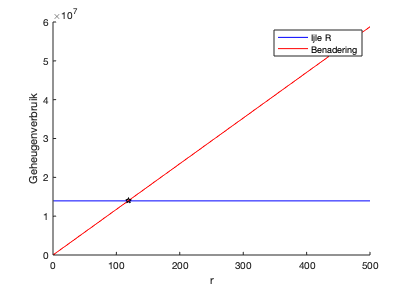
\includegraphics[width=0.3\textwidth]{res/op2.png}
\caption{Geheugenverbruik voor ijle matrix $R$ en lagerangsbenadering. Het snijpunt bevindt zich in $r\approx 119$.}
\label{fig:op2}
\end{figure}

\begin{lstlisting}
[m,n] = size(R);
ratings = nnz(R);
int_mem = 4;
double_mem = 8;
max_r = 500;
%
fprintf('Geheugenruimte full(R) : %i\n', m * n * double_mem)
%
size_sparse_naive = ratings * (int_mem * 2 + double_mem);
size_sparse = 12 * ratings + 4 * n;
fprintf('Geheugenruimte sparse(R) : %i\n', size_sparse)
%
fullR = full(R);
fprintf('Matlab zelf gebruikt respectievelijk %i en %i bytes.\n', whos('fullR').bytes, whos('R').bytes)
%
r = 1:max_r;
size_approx = (m + n) * double_mem * r;
snijpunt_r = size_sparse / ((m + n) * double_mem);
fprintf('Snijpunt in r = %i\n\n', snijpunt_r)
%
hold on
plot(r, repmat(size_sparse,1,max_r), 'b-')
plot(r, size_approx, 'r-')
plot(snijpunt_r, size_sparse, 'kp')
xlabel('r')
ylabel('Geheugenverbruik')
legend('Ijle R', 'Benadering', 'Location', 'northeast') 
\end{lstlisting}

%%%
%%%
%%%

\fakesubsection{Opdracht 3}

Men weet dat 
\begin{equation} \label{eq:1}
A=\sum_{i=1}^r \sigma_iu_iv_i^T \qquad
\end{equation}
Het iteratief algoritme gaat bij elke stap $\sigma_j$, $u_j$ en $v_j$ bepalen zodat de Frobeniusnorm van $E_{j-1}-\sigma_ju_jv_j^T$ (de nieuwe $E_j$) minimaal is. Dit komt overeen met het bepalen van een afgeknotte singulierewaardenontbinding van graad 1. De $\sigma_j$ dient daarbij de grootste singuliere waarde van $E_{j-1}$ te zijn. Stel $j = 0$, dan :
$$E_1=E_0-\sigma_ju_jv_j^T=A-\sigma_ju_jv_j^T=\sum_{i=1}^r \sigma_iu_iv_i^T-\sigma_ju_jv_j^T = \sum_{i=2}^{r} \sigma_iu_iv_i^T$$
Na een aantal iteraties bekomt men uiteindelijk :
$$E_k=\sum_{i=k+1}^{r} \sigma_iu_iv_i^T$$
Want telkens wordt er een afgeknotte singulierewaardenontbinding bepaald van rang 1 en die komt overeen met de term horende bij de grootste singuliere waarde zodat deze term keer op keer verdwijnt na aftrekking. Totdat de laatste $r-k$ termen overblijven. 
Men kan opmerken dat dit niet verreist dat de $u_j$ en $v_j$ bekomen in stap 4 overeenstemmen met de $u_i$ en $v_i$ in (\ref{eq:1}). Het teken van $u_j$ en $v_j$ kan bijvoorbeeld verschillen.\\
\par\noindent Berekent men ten slotte $A-E_k$ dan bekomt men het gevraagde :
$$A-E_k = \sum_{i=1}^{r} \sigma_iu_iv_i^T-\sum_{i=k+1}^{r} \sigma_iu_iv_i^T=\sum_{i=1}^{k} \sigma_iu_iv_i^T$$

\noindent Het algoritme stopt na $k$ stappen (mits men veronderstelt dat $k\leq r$, want anders stop the algoritme vroeger dan dat).

%%%
%%%
%%%

\fakesubsection{Opdracht 4}

Gezien mijn studentennummer $s0216676$ is, is $c$ gelijk aan $6$. Met $sizeof(double)=8$ zal stap 4 een totaal aan $8*(m+n+1)$ bytes nodig hebben. Voor stap 5 krijgt men te maken met de matrix $E$ die maar \'e\'en keer wordt gealloceerd en $8*n*m$ bytes nodig heeft. Stap 6 verbruikt $4$ bytes (voor het geheel getal). Het aantal keren dat men de stappen uitvoert maakt niet uit.\\

\par\noindent Men heeft dus te maken met $((280000+58000+1)*8+(280000*58000*8)+4)/1024^3\approx 120$ GB wat op zich al meer is dan het optimistische $8+2+(c+1)^2=8+2+49=59$ GB.  Als men met ijle voorstellingen blijft werken kan hier iets aan gedaan worden.

%%%
%%%
%%%

\fakesubsection{Opdracht 5}

De drie vectoren \texttt{[i,j,x]} die teruggegeven worden door \texttt{find(A)} verbruiken elk $\mathcal{O}(\zeta)$ geheugen. In de implementatie van de functie \texttt{s0216676\_sparseModel} wordt \texttt{[x]} z\'elf hergebruikt om de resultaten van de lineaire operator $P_{\Omega}(X)$ op te slaan. Elk element $x_{ij}$ is gelijk aan de vermenigvuldiging van rij $i$ van de matrix $Uk*diag(sk)$ en kolom $j$ van $Vk^T$. Het volstaat dus elementsgewijs te vermenigvuldigen van rij $i$ van $Uk$ met $sk^T$ en dit te vermenigvuldigen met de getransponeerde rij $j$ van $Vk$.

\begin{lstlisting}
function [P] = s0216676_sparseModel(Uk,sk,Vk,A)
    [i,j,x] = find(A);
    for idx = 1:nnz(A)
        x(idx) = Uk(i(idx),:) .* sk' * Vk(j(idx),:)';
    end
    P = sparse(i, j, x);
end
\end{lstlisting}

%%%
%%%
%%%

\fakesubsection{Opdracht 6}

Het patroon in de bekomen figuur (figuur \ref{fig:op6}) komt overeen met het ijlheidspatroon van $R$. Dit kan men gebruiken in de volgende opgave. De bekomen matrix $B$ heeft dan al de gewenste structuur en neemt $\mathcal{O}(k\zeta)$ geheugen in.

\begin{figure}[h]
\centering
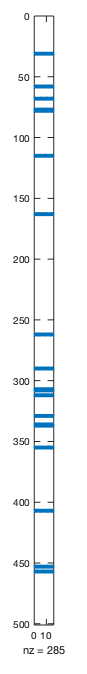
\includegraphics[width=0.1\textwidth]{res/op6.png}
\caption{Resultaat voor opdracht 6. Men herkent het ijlheidspatroon van $R$.}
\label{fig:op6}
\end{figure}

\begin{lstlisting}
B = repmat(spones(R(:)), 1, 15);
spy(B(1:500,:))
\end{lstlisting}

%%%
%%%
%%%

\fakesubsection{Opdracht 7}

Door op voorhand $\mathcal{O}(k\zeta)$ aan geheugen vrij te maken en dan stap voor stap de kolommen van B aan te vullen met de resultaten van de \texttt{sparseModel} functie (die op zijn beurt $\mathcal{O}(\zeta)$ geheugen gebruikt) blijft het geheugengebruik binnen de opgelegde limiet.

\begin{lstlisting}
function [s] = s0216676_optimalCoefficients(Uk,Vk,A)
    B = repmat(spones(A(:)), 1, size(Uk,2));
    for j = 1:size(Uk,2)
        B(:,j) = reshape(s0216676_sparseModel(Uk(:,j), 1, Vk(:,j), A), [], 1);
    end
    [s,~] = lsqr(B, A(:));
end
\end{lstlisting}

%%%
%%%
%%%

\fakesubsection{Opdracht 8}

Om de gemiddelde beoordeling per gebruiker te bekomen wordt de som van al diens beoordelingen genomen en gedeeld door het aantal beoordelingen dat niet nul is. Vervolgens wordt de bekomen ijle vector omgevormd tot een kolomvector.

\begin{lstlisting}
function [mu] = s0216676_userMeans(A)
    mu = (sum(A, 1) ./ sum(A ~= 0))'
end
\end{lstlisting}

%%%
%%%
%%%

\fakesubsection{Opdracht 9}

Er zijn \mcode{length(mu(mu == 5))} (dwz. 13) gebruikers die een gemiddelde beoordeling hebben van 5. De laagste drie gemiddelden bedragen 0.5100, 0.5727 en 0.8983 (\mcode{sort(mu) ; ans(1:3)}).

%%%
%%%
%%%

\fakesubsection{Opdracht 10}

Men kan de \texttt{RMSE} als volgt berekenen :

\begin{lstlisting}
function [err] = s0216676_RMSE(A,B)
    err = norm(A-B, 'fro') / sqrt(nnz(A));
end
\end{lstlisting}

%%%
%%%
%%%

\fakesubsection{Opdracht 11}

De \texttt{RMSE} bedraagt iets meer dan 26 :

\begin{lstlisting}
[i,j] = find(T);
mu = s0216676_userMeans(R);
err = round(s0216676_RMSE(T, sparse(i,j,mu(j))), 4)
% Prints "err = 0.8823"
\end{lstlisting}

%%%
%%%
%%%

\fakesubsection{Opdracht 12}

De \texttt{RMSE} is te zien in figuur \ref{fig:op12}. De volle berekening duurde ongeveer 250 seconden. De reden waarom er divergentie optreedt is dat er \textit{overfitting} is (het model veralgemeent niet goed meer wanneer het de oorspronkelijke data `te goed' benadert).

\begin{figure}[H]
\centering
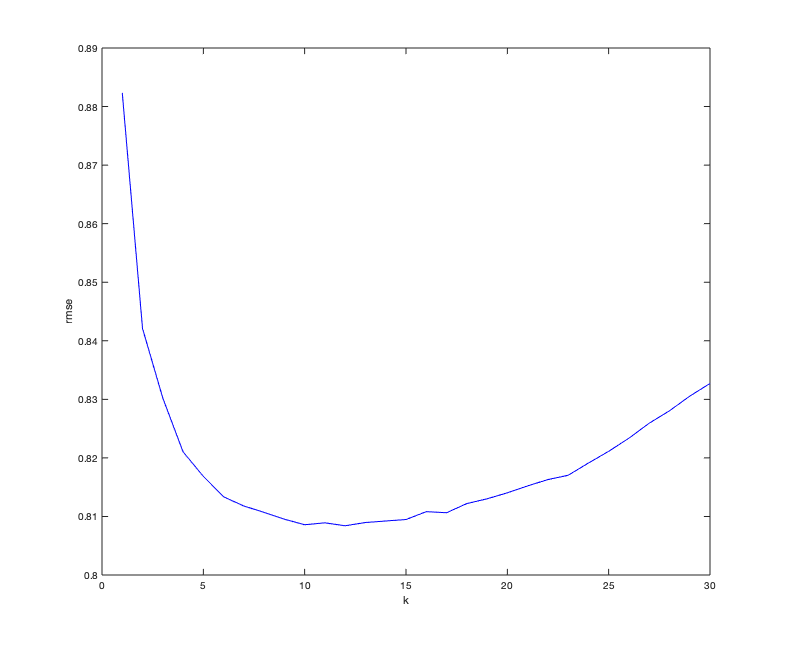
\includegraphics[width=0.5\textwidth]{res/op12.png}
\caption{Resultaat van het algoritme voor $k=30$, toegepast op de MovieLens dataset.}
\label{fig:op12}
\end{figure}

%%%
%%%
%%%

\fakesubsection{Opdracht 13}

De vector $s_{20}$ ziet er als volgt uit :
$$[1.0\ 806.2\ 386.4\ 383.2\ 284.9\ 248.9\ 192.7\ 199.2\ 179.9\ 171.3\ 133.1\ 152.1\ 136.0\ 143.8\ 122.0\ 120.5\ 128.8\ 116.9\ 120.2\ 124.7]$$

%%%
%%%
%%%

\fakesubsection{Opdracht 14}

De functie kan in \'e\'en lijn geschreven worden :

\begin{lstlisting}
function [movieIDs,score] = s0216676_actualBestMovies(R)
    [score,movieIDs] = sort(sum(R,2) ./ sum(R~=0,2), 'descend');
end
\end{lstlisting}

%%%
%%%
%%%

\fakesubsection{Opdracht 15}

Deze keer moet de berekening iteratief gebeuren om het gevraagde maximum aan geheugencomplexiteit te respecteren. De gemiddelde score van elke film wordt apart berekent tot de lijst compleet is. Hierna wordt hij gesorteerd.

\begin{lstlisting}
function [movieIDs,score] = s0216676_predictedBestMovies(Uk,sk,Vk)
    [m,~] = size(Uk); 
    [n,~] = size(Vk);
    score = zeros(n, 1);
    for i = 1:m
        acc = 0;
        x = Uk(i,:) .* sk';
        for j = 1:n
            acc = x * Vk(j,:)' + acc;
        end
        score(i) = acc / n;
    end
    [score, movieIDs] = sort(score, 'descend');
end
\end{lstlisting}

%%%
%%%
%%%

\newgeometry{top=1.5cm,bottom=1.5cm}
\thispagestyle{empty}

\begin{table}[H]
\centering
\begin{tabular}{c|c}
\textbf{Feitelijke beste films} & \textbf{\# beoordelingen} \\
\hline
Planet Earth II (2016)                              &  387 \\
Black Mirror: White Christmas (2014)                &  594 \\
Won't You Be My Neighbor? (2018)                    &   57 \\
Sherlock - A Study in Pink (2010)                   &  131 \\
Blue Planet II (2017)                               &  131 \\
Over the Garden Wall (2013)                         &  218 \\
Whiplash (2013)                                     &  357 \\
Human Planet (2011)                                 &  177 \\
Inception (2010)                                    & 7631 \\
The Night Of (2016)                                 &  184 \\
The Jinx: The Life and Deaths of Robert Durst (2015)&  401 \\
Making a Murderer (2015)                            &  113 \\
Piper (2016)                                        &  631 \\
Frozen Planet (2011)                                &  198 \\
Whiplash (2014)                                     & 3535 \\
Bo Burnham: what. (2013)                            &   95 \\
The Handmaiden (2016)                               &  544 \\
Your Name. (2016)                                   &  605 \\
Story of Film: An Odyssey, The (2011)               &   59 \\
Laurence Anyways (2012)                             &   77 \\
Intouchables (2011)                                 & 3331 \\
Spotlight (2015)                                    & 2264 \\
Winter on Fire: Ukraine's Fight for Freedom (2015)  &   54 \\
John Mulaney: New In Town (2012)                    &  155 \\
O.J.: Made in America (2016)                        &  213\\
\hline
Totaal & 22142 \\
Mediaan & 213
\end{tabular}
\caption{Resultaten van de oproep van functie \texttt{s0216676\_actualBestMovies}.}
\label{fig:op16a}
\end{table}

\begin{table}[H]
\centering
\begin{tabular}{c|c}
\textbf{Voorspelde beste films} & \textbf{\# beoordelingen} \\
\hline
Inception (2010)                & 7631 \\
Whiplash (2014)                 & 3535 \\
Intouchables (2011)             & 3331 \\
Interstellar (2014)             & 6181 \\
Django Unchained (2012)         & 5851 \\
The Martian (2015)              & 5268 \\
Arrival (2016)                  & 3508 \\
Gone Girl (2014)                & 4337 \\
Shutter Island (2010)           & 5505 \\
Grand Budapest Hotel, The (2014)& 4444 \\
Spotlight (2015)                & 2264 \\
Dark Knight Rises, The (2012)   & 6182 \\
King's Speech, The (2010)       & 4225 \\
Ex Machina (2015)               & 4412 \\
The Imitation Game (2014)       & 4614 \\
Big Short, The (2015)           & 2886 \\
Edge of Tomorrow (2014)         & 4807 \\
Inside Out (2015)               & 4549 \\
Prisoners (2013)                & 2360 \\
Guardians of the Galaxy (2014)  & 5700 \\
Her (2013)                      & 3856 \\
Nightcrawler (2014)             & 3139 \\
Room (2015)                     & 1674 \\
Wolf of Wall Street, The (2013) & 5141 \\
Dallas Buyers Club (2013)       & 2747\\
\hline
Totaal & 108147 \\
Mediaan & 4412
\end{tabular}
\caption{Resultaten van de oproep van functie \texttt{s0216676\_predictedBestMovies}.}
\label{fig:op16b}
\end{table}

\restoregeometry

\newpage
\fakesubsection{Opdracht 16}

De `beste films' worden weergegeven in figuur \ref{fig:op16a} en \ref{fig:op16b}. De mediaan voor het aantal beoordelingen bedraagt respectievelijk 213 en 4412. Dus niet alleen ziet de lijst van voorspelde beste films er heel wat realistischer uit, de films hebben ook heel wat meer beoordelingen. Dat maakt de lijst betrouwbaarder.

%%%
%%%
%%%

\fakesubsection{Opdracht 17}

De functie werd als volgt ge\"implementeerd :

\begin{lstlisting}
function [movieIDs,score] = s0216676_predictedBestMoviesForUser(R,Uk,sk,Vk,j)
    [m,~] = size(R);
    indices = setdiff(1:m,find(R))';
    n = length(indices);
    score = zeros(n,1);
    x = sk .* Vk(j,:)';
    for i = 1:n
       score(i) = Uk(indices(i),:) * x;
    end
    [score,permutation] = sort(score, 'descend');
    movieIDs = indices(permutation);
end
\end{lstlisting}

%%%
%%%
%%%

\fakesubsection{Opdracht 18}

De resultaten worden weergegeven in figuur \ref{fig:op18a}, \ref{fig:op18b} en \ref{fig:op18c}.

%\newgeometry{top=1.5cm,bottom=1.5cm}
%\thispagestyle{empty}

\begin{table}[H]
\centering
\begin{tabular}{c|c}
\textbf{Beste films} & \textbf{Score} \\
\hline
    Deadpool (2016)                                   & 5.7072 \\
    The Hunger Games (2012)                           & 4.9250 \\
    Star Wars: Episode VII - The Force Awakens (2015) & 4.8234 \\
    Her (2013)                                        & 4.6669 \\
    The Hunger Games: Mockingjay - Part 1 (2014)      & 4.5391 \\
    Black Swan (2010)                                 & 4.4652 \\
    Perks of Being a Wallflower, The (2012)           & 4.1907 \\
    Scott Pilgrim vs. the World (2010)                & 4.1496 \\
    Avengers: Age of Ultron (2015)                    & 4.1399 \\
    Moonrise Kingdom (2012)                           & 4.0860 
\end{tabular}
\caption{Best beoordeelde films voor gebruiker 98 (op basis van voorspellingen).}
\label{fig:op18a}
\end{table}

\begin{table}[H]
\centering
\begin{tabular}{c|c}
\textbf{Beste films} & \textbf{Score} \\
\hline
    Captain America: The Winter Soldier (2014) & 5.4375 \\
    Deadpool (2016)                            & 5.4323 \\
    Intouchables (2011)                        & 5.3363 \\
    Thor: Ragnarok (2017)                      & 5.3028 \\
    Avengers: Infinity War - Part I (2018)     & 5.2873 \\
    Doctor Strange (2016)                      & 5.2848 \\
    Big Hero 6 (2014)                          & 5.2218 \\
    Logan (2017)                               & 5.1846 \\
    John Wick (2014)                           & 5.0464 \\
    Spotlight (2015)                           & 4.9661 
\end{tabular}
\caption{Best beoordeelde films voor gebruiker 10100 (op basis van voorspellingen).}
\label{fig:op18b}
\end{table}

\begin{table}[H]
\centering
\begin{tabular}{c|c}
\textbf{Beste films} & \textbf{Score} \\
\hline
How to Train Your Dragon (2010)             & 5.0000 \\
The Hunger Games (2012)                     & 5.0000 \\
Dark Knight Rises, The (2012)               & 5.0000 \\
Pitch Perfect (2012)                        & 5.0000 \\
Hobbit: An Unexpected Journey, The (2012)   & 5.0000 \\
Way, Way Back, The (2013)                   & 5.0000 \\
Short Term 12 (2013)                        & 5.0000 \\
Thor: The Dark World (2013)                 & 5.0000 \\
Wolf of Wall Street, The (2013)             & 5.0000 \\
How to Train Your Dragon 2 (2014)           & 5.0000 \\
The Hunger Games: Mockingjay - Part 1 (2014)& 5.0000 \\
Deadpool (2016)                             & 5.0000 \\
Guardians of the Galaxy 2 (2017)            & 5.0000 \\
Sherlock: The Abominable Bride (2016)       & 5.0000 \\
Kubo and the Two Strings (2016)             & 5.0000
\end{tabular}
\caption{Best beoordeelde films voor gebruiker 98 (op basis van testmatrix $T$).}
\label{fig:op18c}
\end{table}

\noindent Voor gebruiker 10100 worden voornamelijk Marvel films aangeraden. Voor gebruiker 98 komen 3 aanbevelingen overeen met diens hoogst-beoordeelde films (in matrix $T$, niet in matrix $R$). De andere films hebben een gelijkaardig genre, dus is wat aangeraden wordt best ok\'e.\\




%
% Evaluatie
%
\appendix
\fakesection{Evaluatie}



% 
% References
%
\bibliographystyle{plain}
\bibliography{references}
\addcontentsline{toc}{section}{Bronnen}

\end{document}
